\documentclass[a4paper]{article}\usepackage[]{graphicx}\usepackage[]{color}
%% maxwidth is the original width if it is less than linewidth
%% otherwise use linewidth (to make sure the graphics do not exceed the margin)
\makeatletter
\def\maxwidth{ %
  \ifdim\Gin@nat@width>\linewidth
    \linewidth
  \else
    \Gin@nat@width
  \fi
}
\makeatother

\definecolor{fgcolor}{rgb}{0.345, 0.345, 0.345}
\newcommand{\hlnum}[1]{\textcolor[rgb]{0.686,0.059,0.569}{#1}}%
\newcommand{\hlstr}[1]{\textcolor[rgb]{0.192,0.494,0.8}{#1}}%
\newcommand{\hlcom}[1]{\textcolor[rgb]{0.678,0.584,0.686}{\textit{#1}}}%
\newcommand{\hlopt}[1]{\textcolor[rgb]{0,0,0}{#1}}%
\newcommand{\hlstd}[1]{\textcolor[rgb]{0.345,0.345,0.345}{#1}}%
\newcommand{\hlkwa}[1]{\textcolor[rgb]{0.161,0.373,0.58}{\textbf{#1}}}%
\newcommand{\hlkwb}[1]{\textcolor[rgb]{0.69,0.353,0.396}{#1}}%
\newcommand{\hlkwc}[1]{\textcolor[rgb]{0.333,0.667,0.333}{#1}}%
\newcommand{\hlkwd}[1]{\textcolor[rgb]{0.737,0.353,0.396}{\textbf{#1}}}%

\usepackage{framed}
\makeatletter
\newenvironment{kframe}{%
 \def\at@end@of@kframe{}%
 \ifinner\ifhmode%
  \def\at@end@of@kframe{\end{minipage}}%
  \begin{minipage}{\columnwidth}%
 \fi\fi%
 \def\FrameCommand##1{\hskip\@totalleftmargin \hskip-\fboxsep
 \colorbox{shadecolor}{##1}\hskip-\fboxsep
     % There is no \\@totalrightmargin, so:
     \hskip-\linewidth \hskip-\@totalleftmargin \hskip\columnwidth}%
 \MakeFramed {\advance\hsize-\width
   \@totalleftmargin\z@ \linewidth\hsize
   \@setminipage}}%
 {\par\unskip\endMakeFramed%
 \at@end@of@kframe}
\makeatother

\definecolor{shadecolor}{rgb}{.97, .97, .97}
\definecolor{messagecolor}{rgb}{0, 0, 0}
\definecolor{warningcolor}{rgb}{1, 0, 1}
\definecolor{errorcolor}{rgb}{1, 0, 0}
\newenvironment{knitrout}{}{} % an empty environment to be redefined in TeX

\usepackage{alltt}
\usepackage{a4wide}
\usepackage[margin=.8in]{geometry}
\usepackage{colortbl}

\title{Comparison of Versions of Kinship Links}
\author{Joe Rodger's BG Team}
\IfFileExists{upquote.sty}{\usepackage{upquote}}{}
\begin{document}
\maketitle

\definecolor{goodColor}{rgb}{.9,1,.85}
\definecolor{sosoColor}{rgb}{1,0.9215686,0.6117647}
\definecolor{badColor}{rgb}{1,.85,.85}
\definecolor{nullColor}{rgb}{.9, 0.85, 0.95} %0.8000000 0.7529412 0.8549020
\setlength{\parindent}{0pt}%http://tex.stackexchange.com/questions/49188/how-to-insert-vertical-space-between-paragraphs







% \textbf{RelationshipPaths Considered}: includedRelationshipPaths;\\
\textbf{Newer Links Version}: 77;
\textbf{Older Links Version}: 76;

\begin{knitrout}
\definecolor{shadecolor}{rgb}{0.969, 0.969, 0.969}\color{fgcolor}\begin{kframe}
\begin{verbatim}
Newer Links: R excludes SameGeneration==0
Older Links: Uses AlwaysLivedWithBothBioparents
\end{verbatim}
\end{kframe}
\end{knitrout}


\begin{figure}[htbp]
\begin{knitrout}
\definecolor{shadecolor}{rgb}{0.969, 0.969, 0.969}\color{fgcolor}
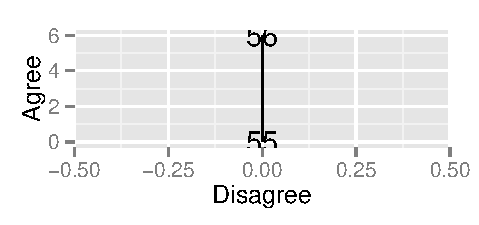
\includegraphics[width=\maxwidth]{figure/unnamed-chunk-31} 

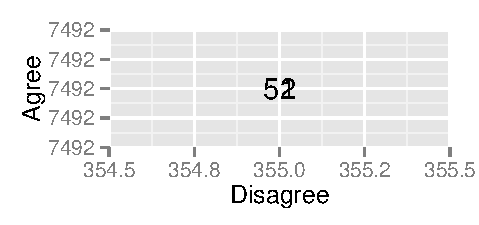
\includegraphics[width=\maxwidth]{figure/unnamed-chunk-32} 

\end{knitrout}

\caption{ROC for Gen1Housemates (left) and Gen2Siblings (right)}
\end{figure}

% latex table generated in R 3.0.2 by xtable 1.7-1 package
% Thu Oct 24 00:06:51 2013
\begin{table}[ht]
\centering
{\large
\begin{tabular}{lrrrrr}
  \hline
R & Implicit2004 & Implicit & Roster & Explicit & Eventual \\ 
  \hline
0 & - &  82 & 478 &  41 & 539 \\ 
  0.0625 & - & - & - &   2 &  47 \\ 
  0.125 &  76 & - &  96 & - &  96 \\ 
  0.25 &  43 &  33 & - & 273 & 274 \\ 
  0.375 & 310 & - & - &  37 &  15 \\ 
  0.5 & 1877 & 3771 & - & 3598 & 4045 \\ 
  0.75 &  32 & - & - & - &  11 \\ 
  1 & - & - & - & - &  11 \\ 
  - & 2964 & 1416 & 4728 & 1351 & 264 \\ 
   \hline
\end{tabular}
}
\caption{Counts for Gen1Housemates} 
\end{table}
% latex table generated in R 3.0.2 by xtable 1.7-1 package
% Thu Oct 24 00:06:51 2013
\begin{table}[ht]
\centering
{\large
\begin{tabular}{lrrrrr}
  \hline
R & Implicit2004 & Implicit & Roster & Explicit & Eventual \\ 
  \hline
0 & - &  82 & 478 &  41 & 539 \\ 
  0.0625 & - & - & - &   2 &  47 \\ 
  0.125 &  76 & - &  96 & - &  96 \\ 
  0.25 &  43 &  33 & - & 273 & 274 \\ 
  0.375 & 310 & - & - &  37 &  15 \\ 
  0.5 & 1877 & 3771 & - & 3598 & 4045 \\ 
  0.75 &  32 & - & - & - &  11 \\ 
  1 & - & - & - & - &  11 \\ 
  - & 2964 & 1416 & 4728 & 1351 & 264 \\ 
   \hline
\end{tabular}
}
\caption{Counts for Gen1Housemates (Previous version of links)} 
\end{table}
% latex table generated in R 3.0.2 by xtable 1.7-1 package
% Thu Oct 24 00:06:51 2013
\begin{table}[ht]
\centering
{\large
\begin{tabular}{lrrrr}
  \hline
R & Implicit2004 & Implicit & Explicit & Eventual \\ 
  \hline
- &   0 &   0 &   0 &   0 \\ 
   \hline
\end{tabular}
}
\caption{Counts for Gen2Siblings} 
\end{table}
% latex table generated in R 3.0.2 by xtable 1.7-1 package
% Thu Oct 24 00:06:51 2013
\begin{table}[ht]
\centering
{\large
\begin{tabular}{lrrrr}
  \hline
R & Implicit2004 & Implicit & Explicit & Eventual \\ 
  \hline
- &   0 &   0 &   0 &   0 \\ 
   \hline
\end{tabular}
}
\caption{Counts for Gen2Siblings (Previous version of links)} 
\end{table}



% latex table generated in R 3.0.2 by xtable 1.7-1 package
% Thu Oct 24 00:06:51 2013
\begin{table}[ht]
\centering
\begin{tabular}{rrrrrr}
  \hline
Count & RImplicit2004 & RImplicit & RExplicit & RRoster & Delta \\ 
  \rowcolor{goodColor}  \hline
1477 & 0.500 & 0.500 & 0.500 & - & 0 \\ 
   \rowcolor{goodColor} 1287 & - & 0.500 & 0.500 & - & 0 \\ 
   \rowcolor{sosoColor} 501 & - & - & 0.500 & - & 0 \\ 
   \rowcolor{nullColor} 244 & - & - & - & - & 0 \\ 
  236 & - & 0.500 & - & - & 0 \\ 
  215 & 0.500 & 0.500 & - & - & 0 \\ 
  198 & - & 0.500 & - & 0.000 & 0 \\ 
   \rowcolor{sosoColor} 177 & 0.375 & - & 0.500 & - & 0 \\ 
   \rowcolor{sosoColor} 148 & - & - & 0.250 & - & 0 \\ 
  100 & 0.500 & 0.500 & - & 0.000 & 0 \\ 
   \rowcolor{nullColor} 99 & - & - & - & 0.000 & 0 \\ 
   \rowcolor{badColor} 71 & - & 0.500 & 0.250 & - & 0 \\ 
   \rowcolor{nullColor} 41 & 0.375 & - & - & - & 0 \\ 
   \rowcolor{goodColor} 39 & 0.375 & 0.500 & 0.500 & - & 0 \\ 
  29 & 0.125 & 0.500 & - & 0.125 & 0 \\ 
   \rowcolor{sosoColor} 27 & 0.500 & - & 0.500 & - & 0 \\ 
  25 & - & 0.000 & - & 0.000 & 0 \\ 
   \rowcolor{nullColor} 19 & 0.125 & - & - & 0.125 & 0 \\ 
  19 & - & 0.000 & - & - & 0 \\ 
   \rowcolor{badColor} 18 & 0.500 & 0.500 & 0.250 & - & 0 \\ 
   \rowcolor{sosoColor} 18 & - & - & 0.000 & - & 0 \\ 
   \rowcolor{sosoColor} 17 & 0.375 & - & 0.250 & - & 0 \\ 
   \rowcolor{nullColor} 15 & 0.500 & - & - & - & 0 \\ 
   \rowcolor{sosoColor} 15 & - & - & 0.375 & - & 0 \\ 
  14 & - & 0.500 & - & 0.125 & 0 \\ 
   \rowcolor{sosoColor} 13 & 0.250 & - & 0.500 & - & 0 \\ 
   \rowcolor{goodColor} 12 & 0.750 & 0.500 & 0.500 & - & 0 \\ 
  11 & - & 0.500 & 0.375 & - & 0 \\ 
   \rowcolor{sosoColor} 10 & 0.125 & - & 0.500 & - & 0 \\ 
   \rowcolor{nullColor} 10 & - & - & - & 0.125 & 0 \\ 
   \rowcolor{badColor} 9 & - & 0.500 & 0.000 & - & 0 \\ 
   \rowcolor{nullColor} 8 & 0.250 & - & - & 0.000 & 0 \\ 
   \rowcolor{nullColor} 8 & 0.250 & - & - & - & 0 \\ 
   \rowcolor{badColor} 8 & 0.500 & 0.250 & 0.500 & - & 0 \\ 
   \rowcolor{badColor} 8 & - & 0.000 & 0.500 & - & 0 \\ 
   \rowcolor{goodColor} 7 & 0.250 & 0.500 & 0.500 & - & 0 \\ 
   \rowcolor{sosoColor} 7 & 0.750 & - & 0.500 & - & 0 \\ 
   \rowcolor{badColor} 7 & - & 0.250 & 0.500 & - & 0 \\ 
   \rowcolor{badColor} 5 & 0.375 & 0.000 & 0.500 & - & 0 \\ 
  5 & 0.375 & 0.500 & - & - & 0 \\ 
   \rowcolor{nullColor} 5 & 0.375 & - & - & 0.000 & 0 \\ 
  5 & 0.500 & 0.500 & 0.375 & - & 0 \\ 
   \rowcolor{nullColor} 5 & 0.750 & - & - & - & 0 \\ 
   \rowcolor{badColor} 5 & - & 0.000 & 0.250 & - & 0 \\ 
  5 & - & 0.000 & - & 0.125 & 0 \\ 
  5 & - & 0.250 & - & 0.000 & 0 \\ 
  5 & - & 0.250 & - & 0.125 & 0 \\ 
   \rowcolor{goodColor} 4 & 0.125 & 0.500 & 0.500 & - & 0 \\ 
  4 & 0.375 & 0.000 & - & 0.000 & 0 \\ 
  4 & 0.375 & 0.500 & - & 0.000 & 0 \\ 
   \rowcolor{sosoColor} 4 & 0.375 & - & 0.375 & - & 0 \\ 
   \rowcolor{nullColor} 3 & 0.125 & - & - & 0.000 & 0 \\ 
   \rowcolor{nullColor} 3 & 0.125 & - & - & - & 0 \\ 
  3 & 0.750 & 0.500 & - & 0.000 & 0 \\ 
  3 & 0.750 & 0.500 & - & - & 0 \\ 
   \rowcolor{goodColor} 3 & - & 0.000 & 0.000 & - & 0 \\ 
   \rowcolor{badColor} 3 & - & 0.500 & 0.250 & 0.000 & 0 \\ 
   \rowcolor{goodColor} 3 & - & 0.500 & 0.500 & 0.000 & 0 \\ 
   \rowcolor{badColor} 2 & 0.125 & 0.500 & 0.000 & - & 0 \\ 
  2 & 0.250 & 0.500 & - & 0.000 & 0 \\ 
   \rowcolor{sosoColor} 2 & 0.250 & - & 0.250 & - & 0 \\ 
  2 & 0.375 & 0.000 & - & 0.125 & 0 \\ 
  2 & 0.375 & 0.000 & - & - & 0 \\ 
   \rowcolor{nullColor} 2 & 0.375 & - & - & 0.125 & 0 \\ 
  2 & 0.500 & 0.250 & - & 0.000 & 0 \\ 
   \rowcolor{badColor} 2 & 0.500 & 0.500 & 0.000 & - & 0 \\ 
   \rowcolor{nullColor} 2 & 0.750 & - & - & 0.000 & 0 \\ 
   \rowcolor{goodColor} 2 & - & 0.250 & 0.250 & - & 0 \\ 
   \rowcolor{badColor} 2 & - & 0.500 & 0.000 & 0.000 & 0 \\ 
   \rowcolor{badColor} 2 & - & 0.500 & 0.000 & 0.125 & 0 \\ 
   \rowcolor{sosoColor} 2 & - & - & 0.250 & 0.000 & 0 \\ 
   \rowcolor{sosoColor} 2 & - & - & 0.500 & 0.000 & 0 \\ 
  1 & 0.125 & 0.000 & - & - & 0 \\ 
  1 & 0.125 & 0.250 & - & 0.125 & 0 \\ 
   \rowcolor{badColor} 1 & 0.125 & 0.500 & 0.000 & 0.125 & 0 \\ 
   \rowcolor{sosoColor} 1 & 0.125 & - & 0.000 & - & 0 \\ 
   \rowcolor{sosoColor} 1 & 0.125 & - & 0.250 & - & 0 \\ 
   \rowcolor{sosoColor} 1 & 0.125 & - & 0.500 & 0.125 & 0 \\ 
  1 & 0.250 & 0.000 & - & 0.000 & 0 \\ 
  1 & 0.250 & 0.500 & - & - & 0 \\ 
   \rowcolor{nullColor} 1 & 0.250 & - & - & 0.125 & 0 \\ 
   \rowcolor{goodColor} 1 & 0.375 & 0.000 & 0.000 & 0.000 & 0 \\ 
   \rowcolor{badColor} 1 & 0.375 & 0.500 & 0.250 & - & 0 \\ 
   \rowcolor{goodColor} 1 & 0.375 & 0.500 & 0.500 & 0.000 & 0 \\ 
  1 & 0.500 & 0.250 & - & 0.125 & 0 \\ 
  1 & 0.500 & 0.250 & - & - & 0 \\ 
   \rowcolor{badColor} 1 & 0.500 & 0.500 & 0.062 & - & 0 \\ 
   \rowcolor{goodColor} 1 & 0.500 & 0.500 & 0.500 & 0.000 & 0 \\ 
  1 & 0.500 & 0.500 & - & 0.125 & 0 \\ 
   \rowcolor{sosoColor} 1 & 0.500 & - & 0.250 & - & 0 \\ 
   \rowcolor{sosoColor} 1 & 0.500 & - & 0.375 & - & 0 \\ 
   \rowcolor{nullColor} 1 & 0.500 & - & - & 0.000 & 0 \\ 
   \rowcolor{badColor} 1 & - & 0.000 & 0.375 & - & 0 \\ 
   \rowcolor{goodColor} 1 & - & 0.250 & 0.250 & 0.000 & 0 \\ 
   \rowcolor{badColor} 1 & - & 0.500 & 0.250 & 0.125 & 0 \\ 
   \rowcolor{sosoColor} 1 & - & - & 0.062 & - & 0 \\ 
   \rowcolor{sosoColor} 1 & - & - & 0.500 & 0.125 & 0 \\ 
   \hline
\end{tabular}
\caption{Counts for Gen1Housemates} 
\end{table}



\end{document}
